\setchaptergraphic{
    \begin{tikzpicture}[
        shorten >=1pt,>={Stealth[round]},
        node distance=2.5 cm,
        every state/.style={draw=blue!50,very thick,fill=blue!20}
    ]
        \node[initial, state]   (A)                    {$q_0$};
        \node[state, accepting] (B) [right of=A]       {$q_1$};
        \node[state, accepting] (C) [above right of=B] {$q_2$};
        \node[state]            (R) [below right of=B] {$q_3$};

        \path[->] (A) edge [above]                  node [align=center] {0,1} (B)
                  (B) edge [above left, bend left]  node [align=center] {1} (C)
                      edge [below left]             node [align=center] {0} (R)
                  (C) edge [below right, bend left] node [align=center] {0,1} (B)
                  (R) edge [loop right]             node [align=center] {0,1} ();
    \end{tikzpicture}
}

\chapter{Computation Theory}
\label{ch:computation}

\section{Finite Automata}

\begin{defn}
    An \emph{alphabet} is a non-empty set whose elements are referred to as \emph{symbols}. \emph{Strings} (or \emph{words}) over a given alphabet are finite sequences of symbols from the alphabet. A \emph{language} is a set of strings over an alphabet.
\end{defn}

\begin{rmk}
    Alphabets and languages may be non-finite, but strings are generally considered to only include finite sequences. The empty string will be denoted by $\emptystring$.
\end{rmk}

\begin{defn}
    Let $\Sigma$ be an alphabet. Then the language consisting of all strings over $\Sigma$ of length $n$ is denoted by $\Sigma^{n}$. The \emph{Kleene closure} of $\Sigma$ is
    \begin{align*}
        \Sigma^{*} = \bigunion_{i\in\N}\Sigma^{i}.
    \end{align*}
\end{defn}

\begin{defn}
    Given languages $A$ and $B$, the \emph{concatenation} of $A$ and $B$, denoted by $A \concat B$, is
    \begin{align*}
        A \concat B = \left\{\alpha\beta : \alpha \in A, \beta \in B \right\},
    \end{align*}
    where $\alpha\beta$ is the string formed by concatenating $\alpha$ and $\beta$.
\end{defn}

\begin{defn}
    Let $L$ be a language. We can also apply the Kleene star operator to this language, creating its Kleene closure $L^*$ by defining
    \begin{align*}
        L^0 &= \{\emptystring\}, \\
        L^{i+1} &= L^{i} \concat L, \\
        L^{*} &= \bigunion_{i \geq 0}L^{i}.
    \end{align*}
\end{defn}

\begin{defn}
    A (deterministic) \emph{finite automaton} is a $5$-tuple $(Q, \Sigma, \delta, q_0, F)$, where
    \begin{itemize}
        \item $Q$ is a finite set of \emph{states},
        \item $\Sigma$ is an alphabet,
        \item $\delta: Q \times \Sigma \to Q$ is the \emph{transition function},
        \item $q_0 \in Q$ is the \emph{start state},
        \item $F \subseteq Q$ are the \emph{accept states}.
    \end{itemize}
    An automaton starts in state $q_0$, and is given an input consisting over a string over $\Sigma$. For each symbol $s$ in the input, the automaton moves from state $q$ to state $\delta(q, s)$. Once the end of the input is reached, if the state $q$ of the automaton is an accept state --- that is, $q \in F$, then the automaton is said to have \emph{accepted} the input.
\end{defn}

\begin{defn}
    The \emph{language accepted by} a finite automaton $M$ is a language $A$ consisting of all strings over $\Sigma$ that are accepted by the finite automaton. We denote this by $L(M) = A$. A \emph{regular language} is any language accepted by some finite automaton.
\end{defn}

\begin{rmk}
    Finite automata can be represented as a graph, where states are represented as nodes, and transitions are edges between states, labelled by the symbol that triggers the transition. When graphically representing a finite automaton as a graph, accept states may be represented as double-circled nodes.
\end{rmk}

\begin{exmp}
    \begin{figure}[ht!]
        \centering
        \begin{tikzpicture}[
            shorten >=1pt,>={Stealth[round]},
            node distance=2 cm,
            every state/.style={draw=blue!50,very thick,fill=blue!20}
        ]
            \node[initial, state]   (S) {$q_0$};
            \node[state]            (0) [right of=S] {$q_1$};
            \node[state]            (00) [right of=0] {$q_2$};
            \node[state, accepting] (001) [right of=00] {$q_3$};
    
            \path[->] (S)   edge [above, bend left]     node [align=center] {0} (0)
                      (S)   edge [loop below]           node [align=center] {1} ()
                      (0)   edge [above, bend left]     node [align=center] {0} (00)
                            edge [above, bend left]     node [align=center] {1} (S)
                      (00)  edge [loop above]           node [align=center] {0} ()
                            edge [above, bend left]     node [align=center] {1} (001)
                      (001) edge [below, bend left]     node [align=center] {0} (0)
                            edge [above, bend right=60] node [align=center] {1} (S);
        \end{tikzpicture}
        \caption{Example finite automaton}
        \label{fig:example-finite-automaton}
    \end{figure}

    In the finite automaton shown in Figure \ref{fig:example-finite-automaton}, $Q = \left\{q_0, q_1, q_2, q_3\right\}$, $\Sigma = \left\{0, 1\right\}$, $F = \{q_3\}$, and $\delta$ is
    \begin{center}
        \begin{tabular}{|c||c|c|}
            \hline
            \thead{$\delta$} & \thead{$0$}    & \thead{$1$} \\
            \hline\hline
            \textsc{$q_0$}   & \textsc{$q_1$} & \textsc{$q_0$} \\
            \hline
            \textsc{$q_1$}   & \textsc{$q_2$} & \textsc{$q_0$} \\
            \hline
            \textsc{$q_2$}   & \textsc{$q_2$} & \textsc{$q_3$} \\
            \hline
            \textsc{$q_3$}   & \textsc{$q_1$} & \textsc{$q_0$} \\
            \hline
        \end{tabular}.
    \end{center}

    This language accepted by this finite automaton is the set of all binary strings which end with \texttt{001}. We can use an inductive proof on the length of the longest input to prove this.
\end{exmp}

\begin{prop}\label{regular-language-complement}
    Let $A$ be a regular language, then $\complementof{A}$ is also a regular lanaguage.
\end{prop}

\begin{proof}
    Let $M = (Q, \Sigma, \delta, s_0, F)$ be a finite automaton that recognizes $A$, and define
    \begin{align*}
        M' = (Q, \Sigma, \delta, s_0, Q \setminus F).
    \end{align*}
    For any $w \in \Sigma^{*}$, we can see that $M$ and $M'$ reach the same final state, let this be $s_f$. Since $s_f \in F$ if and only if $s_f \in Q \setminus F$, it follows that $M'$ accepts $w$ if and only if $M$ \emph{does not}, therefore the regular language that $M'$ recognizes is precisely $\complementof{A}$.
\end{proof}

\begin{thm}\label{regular-language-union-intersection}
    Let $A$ and $B$ be regular languages, then $A \union B$ and $A \intersection B$ are also regular languages.
\end{thm}

\begin{proof}
    Let $\Sigma$ be the union of the alphabets of $A$ and $B$. Since $A$ and $B$ are regular, we know that there exists finite automata $M_A = \left(Q_1, \Sigma, \delta_1, s_1, F_1\right)$ and $M_B = \left(Q_2, \Sigma, \delta_2, s_2, F_2\right)$. Now we construct a new finite automaton that runs $M_A$ and $M_B$ in parallel. To do this, consider the finite automaton $M = \left(Q, \Sigma, \delta, s, F\right)$, where $Q = Q_1 \times Q_2$, $s = (s_1, s_2)$, and  $\delta: (Q_1 \times Q_2) \times \Sigma \to Q_1 \times Q_2$ is defined by $\delta\left((p_1, p_2), a\right) = \left(\delta_1\left(p_1, a\right), \delta_2\left(p_2, a\right)\right)$.
    
    If $F = F_1 \times F_2$, then $M$ accepts precisely the strings accepted by both $M_A$ and $M_B$ --- that is, $L(M) = A \intersection B$. If instead $F = \left(F_1 \times Q_2\right) \union \left(Q_1 \times F_2\right)$, then $M$ accepts the strings accepted by at least one of $M_A$ and $M_B$ --- that is, $L(M) = A \union B$.
\end{proof}

\begin{defn}
    A \emph{non-deterministic} finite automaton is a $5$-tuple $(Q, \Sigma, \delta, q_0, F)$, where
    \begin{itemize}
        \item $Q$ is a finite set of \emph{states},
        \item $\Sigma$ is an alphabet,
        \item $\delta: Q \times \left(\Sigma \union \{\emptystring\}\right) \to 2^{Q}$ is the \emph{transition function},
        \item $q_0 \in Q$ is the \emph{start state},
        \item $F \subseteq Q$ are the \emph{accept states}.
    \end{itemize}
    A non-deterministic finite automaton $M$ accepts an input $w$ over $\Sigma$ when there exists $w_{\emptystring}$ that causes $M$ to end in an accept state, where $w_{\emptystring}$ is constructed by inserting any finite number of $\emptystring$ into $w$.
\end{defn}

\begin{rmk}
    Standard deterministic finite automata may be referred to as DFAs, while non-deterministic finite automata may be referred to as NFAs.
\end{rmk}

\begin{rmk}
    A NFA can essentially be viewed as a DFA which can split into multiple parallel copies of itself.
\end{rmk}

\begin{defn}
    Given a transition function $\delta: Q \times \left(\Sigma \union \{\emptystring\}\right) \to 2^{Q}$ and $R \subseteq Q$,
    the \emph{$\emptystring$-closure} of $R$ is the set of all states reachable from $R$ via zero or more \emph{$\emptystring$-transitions}. Formally, we recursively define
    \begin{align*}
        E_0\left(R\right) &= R, \\
        E_{i+1}\left(R\right) &= \left\{q \in Q : \exists r \in E_{i}\left(R\right)\left[q \in \delta\left(r, \emptystring\right)\right]\right\}.
    \end{align*}
    and then the $\emptystring$-closure of $R$ is
    \begin{align*}
        E\left(R\right) = \bigunion_{0\leq i < n}E_{i}\left(R\right),
    \end{align*}
    where $n = \abs{Q}$.
\end{defn}

\begin{lemma}\label{epsilon-closure}
    Consider an NFA with states $Q$ and transition function $\delta$, and consider $s\in Q$ and $R \subseteq Q$. Then $s \in E(R)$ if and only if $s$ is reachable from some $q \in R$ via zero or more $\emptystring$-transitions.
\end{lemma}

\begin{proof}\proofbreak
    ($\implies$) If $s \in E(R)$, then $s \in E_{i}(R)$ for some $0 \leq i < n$. If $i = 0$, then $s \in R$ and so $s$ is reachable from $q = s \in R$ via zero $\emptystring$-transitions. If $i > 0$, then there exists $r \in E_{i=1}(R)$ such that $s \in \delta(r, \emptystring)$, and so by induction there exists $q \in R$ such that $s$ is reachable from $q$ via zero or more $\emptystring$-transitions.

    ($\impliedby$) If $s$ is reachable from $q_0 \in R$ via zero of more $\emptystring$-transitions, then clearly there exists a sequence $q_0, q_1, \ldots, q_{k}, s$ such that $q_{i+1} \in \delta(q_i, \emptystring)$ and $s \in \delta(q_k, \emptystring)$. Therefore, $q_i \in E_i(R)$, and so $s \in E_{k+1}$. Notice that if $q_i = q_j$, we can take reach $s$ from $q_0$ via the subsequence $q_0, q_1, \ldots, q_i, q_{j+1}, q_{j+2}, \ldots, q_k, s$. Since $n = \abs{Q}$, it follows by the pigeonhole principle that such a sequence with at most $n$ states must exist, and so $k + 2 \leq n$, which in turn implies $s \in E_{i = k+1}(R)$ for some $0 \leq i < n$, and so $s \in E(R)$.
\end{proof}

\begin{lemma}\label{epsilon-closure-union}
    Consider an NFA with states $Q$ and transition function $\delta$, and consider $A \subseteq Q$ and $B \subseteq Q$. Then
    \begin{align*}
        E(A) \union E(B) = E(A \union B).
    \end{align*}
\end{lemma}

\begin{proof}
    If $x \in E(A) \union E(B)$, then since $A$ and $B$ are arbitrary we have without loss of generality that $x \in E(A)$. It follows by Lemma \ref{epsilon-closure} that $x$ is reachable via $\emptystring$-transitions from some $a \in A$, and since $a \in A \union B$ we then have $x \in E(\union B)$.

    If $x \in E(A \union B)$, then by Lemma \ref{epsilon-closure} we know that $x$ is reachable via $\emptystring$-transitions from some $a \in A$ or some $b \in B$. Then $x \in E(A)$ or $x \in E(B)$, and so $x \in E(E) \union E(B)$.
\end{proof}

\begin{thm}\label{dfa-nfa-equivalence}
    Let $N$ be a non-deterministic finite automaton, and $L$ be the language it accepts. Then $L$ is a regular language. Equivalently, there is an equivalent deterministic finite automaton for every non-deterministic finite automaton.
\end{thm}

\begin{proof}
    Let $V = \left(Q, \Sigma, \delta, q_0, F\right)$ be a non-deterministic finite automaton. We will construct an equivalent deterministic finite automaton $M$. Let $M = \left(Q', \Sigma, \delta', q_0', F'\right)$, where
    \begin{itemize}
        \item $Q' = 2^Q$,
        \item For all $R \in Q'$, define $\delta'(R, a) = E\left(\bigunion_{r \in R}\delta(r, a)\right)$,
        \item $q_0' = \left\{q_0\right\}$,
        \item $F' = \left\{R \in Q \compbar R \intersection F \neq \emptyset\right\}$.
    \end{itemize}

    For any $w \in \Sigma^*$ such that $V$ accepts $w$, by we can construct $w_{\emptystring}$ from $w$ by inserting some number of $\emptystring$'s into $w$ such that $w_{\emptystring}$ causes $V$ to run to an accept state. Let $q_0, q_1, \ldots, q_n$ be the states that $w_{\emptystring}$ causes $V$ to visit. I claim that if $V$ is in state $q_i$ after seeing $w_1, \ldots, w_i$ then $M$ is in state $R$ where $q_i \in R$. We will prove this by induction. The base case is true by construction since $V$ starts in state $q_0$ and $M$ in state $\{q_0\}$. The induction step simply amounts to showing that if $q_i \in R$ then $q_{i+1} \in \delta'(R, w_{i+1})$.
    \begin{align*}
        R' = \delta'(R, w_{i+1}) = E\left(\bigunion_{r\in R}\delta(r, w_{i+1})\right).
    \end{align*}
    Since $w_i$ causes $V$ to move from $q_i$ to $q_{i+1}$, it follows that there is a (possibly empty) sequence of $\emptystring$-transitions from $q_i$ to some state $a$, then $d \in \delta(a, w_i)$, and then a (again possibly empty) sequence of $\emptystring$-transitions from $d$ to $q_{i+1}$. By Lemma \ref{epsilon-closure}, we know that $a \in R$, and therefore $d \in \bigunion_{r \in R}\delta(r, w_i)$, and so again using Lemma \ref{epsilon-closure} we can conclude that $q_{i+i} \in R'$.

    We have therefore shown that $q_n \in R_f$, where $R_f$ is the final state of $M$. Since $V$ accepts $w$ we know that $q_n \in F$ and so $R_f \intersection F \neq \empty$ which implies $R_f \in F'$, and so $M$ also accepts $w$.

    Now consider instead $w$ accepted by $M$. Let $R_0 = \{q_0\}, R_1, \ldots, R_n$ be the sequence of states visited by $M$. Since $w$ is accepted by $M$, we know $R_n \intersection F \neq \emptyset$, so take $q_n \in R_n \intersection F$. It follows that there exists some $q_{n-1} \in R_{n-1}$ such that $q_n \in E(\delta(q_{n-1}, w_{i+1}))$ by Lemmas \ref{epsilon-closure} and \ref{epsilon-closure-union}, and so inductively there must exist a sequence of states of $V$ $q_0, \ldots, q_n$ such that $q_n \in F$ and $q_{i+1}$ is reachable from $q_i$ via $w_i$ and some number of $\emptystring$-transitions. Let $w_{\emptystring}$ be constructed from $w$ by inserting the relevant $\emptystring$'s, and then $w_{\emptystring}$ causes $V$ to end in an accept state, and so $w$ is accepted by $V$ by definition.
\end{proof}

\begin{rmk}
    In addition to a proof of the equivalence of deterministic and non-deterministic finite automata, this is an explicit method to construct a deterministic finite automaton from a non-deterministic one.
\end{rmk}

\begin{thm}\label{regular-language-concatenation}
    Let $A$ and $B$ be regular languages, then $A \concat B$ is also regular.
\end{thm}

\begin{proof}
    Let $A = (Q_A, \Sigma, \delta_A, q_A, F_A)$ and $B = (Q_B, \Sigma, \delta_B, q_B, F_B)$ be deterministic finite automata recognizing language $A$ and $B$ respectively. We now construct a non-deterministic finite automaton which recognizes $A \concat B$. Consider $M = \left(Q, \Sigma, \delta, q_0, F\right)$, where
    \begin{itemize}
        \item $Q = Q_A \union Q_B$,
        \item For $a \in \Sigma$, define $\delta(q, a) = \begin{dcases}
            \{\delta_A(q, a)\}, &q \in Q_A \\
            \{\delta_B(q, a)\}, &q \in Q_B \\
        \end{dcases}$ and $\delta(q, \emptystring) = \begin{dcases}
            \{q_B\}, &q \in F_A \\
            \emptyset, &\textrm{otherwise} \\
        \end{dcases}$,
        \item $q_0 = q_A$,
        \item $F = F_B$.
    \end{itemize}
    Notice that if $w = \alpha\beta$, then the input $\alpha\emptystring\beta$ will cause $M$ to end in an accept state, and so any such $w$ is accepted. If $w$ is accepted, then since the only transition possible from states in $Q_A$ to those in $Q_B$ (which contains all possible accept states) is an $\emptystring$-transition from a state in $F_A$, and so $w = \alpha\beta$ for some $\alpha \in A$ and $\beta \in B$.

    Since $M$ recognizes $A \concat B$, by Theorem \ref{dfa-nfa-equivalence} we know that $A \concat B$ must be a regular language.
\end{proof}

\begin{thm}\label{regular-language-kleene-star}
    Let $A$ be a regular language, then $A^{*}$ is also regular.
\end{thm}

\begin{proof}
    Given a deterministic finite automaton $M = (Q, \Sigma, \delta, q_0, F)$, we make a number of small modifications in order to produce a non-deterministic finite automaton $N$ recognizing $A^{*}$ and thus proving it is regular. Specifically, we add $\emptystring$-transitions from every accept state of $M$ back to $q_0$ --- this allows $N$ to recognize any string you can form by concatenating strings from $A$. We also introduce a new start state with a single $\emptystring$-transition to the original start state, and make this new start state an accept state, thus allowing $N$ to also recognize $\emptystring$.

    Formally, we define $N = (Q_N, \Sigma, \delta_N, q_N, F_N)$ where
    \begin{itemize}
        \item $Q_N = Q \union \{q_N\}$,
        \item $\delta_N(q, a) = \begin{dcases}
            \delta(q, a), &q \in Q \\
            \{\}, &q = q_N \\
        \end{dcases}$ and $\delta_N(q, \emptystring) = \begin{dcases}
            \delta(q, \emptystring) \union \{q_0\}, &q \in F, q \neq q_N \\
            \delta(q, \emptystring), &q \not\in F, q \neq q_N \\
            \{q_0\}, &q = q_N \\
        \end{dcases}$,
        \item $F_N = F \union \{q_N\}$.
    \end{itemize}
\end{proof}

\begin{defn}
    The \emph{regular operations} are union, intersection, complement, concatenation, and star, under which we have shown the set of regular languages is closed.
\end{defn}

\section{Regular Expressions}

\begin{defn}
    A \emph{regular expression} is a sequence of regular operations applied to regular languages. Formally, given an alphabet $\Sigma$, we recursively define the regular expressions over $\Sigma$ as:
    \begin{itemize}
        \item $a$, for any $a \in \Sigma$,
        \item $\emptystring$,
        \item $\emptyset$,
        \item $R_1 \union R_2$, where $R_1$ and $R_2$ are themselves regular expressions,
        \item $R_1 \concat R_2$, where $R_1$ and $R_2$ are themselves regular expressions,
        \item $R_1^{*}$, where $R_1$ is a regular expression,
    \end{itemize}
\end{defn}

\begin{defn}
    For a regular expression $R_1$, we also define $R_1^{+} = R_1R_1^{*}$.
\end{defn}

\begin{exmp}
    The regular expression $\{1\}^{*}(\{0\} \concat \{1\}^{+})^{*}$, also written in a more condensed form as $1^{*}(01^{+})^{*}$, is the language of consisting of binary strings where every $0$ is followed by at least one $1$.
\end{exmp}

\begin{lemma}\label{regex-to-regular-language}
    The language described by any regular expression is a regular language.
\end{lemma}

\begin{proof}
    Let $R$ be a regular expression that describes a language $L$ over an alphabet $\Sigma$. We recursively construct a non-deterministic finite automaton that recognizes $L$ in order to prove that $L$ must be regular. First, any regular expression by definition must have one of the six forms listed in our definition.

    If $R = a$, then $L = \{a\}$ by definition, which is recognized by the non-deterministic finite automaton:
    \begin{figure}[ht!]
        \centering
        \begin{tikzpicture}[
            shorten >=1pt,>={Stealth[round]},
            node distance=2 cm,
            every state/.style={draw=blue!50,very thick,fill=blue!20}
        ]
            \node[initial, state]   (S)              {$q_1$};
            \node[state, accepting] (A) [right of=S] {$q_2$};
    
            \path[->] (S) edge [above] node [align=center] {a} (A);
        \end{tikzpicture}
    \end{figure}

    If $R = \emptystring$, it can be recognized by the non-deterministic finite automaton:
    \begin{figure}[ht!]
        \centering
        \begin{tikzpicture}[
            shorten >=1pt,>={Stealth[round]},
            node distance=2 cm,
            every state/.style={draw=blue!50,very thick,fill=blue!20}
        ]
            \node[initial, state, accepting] (S) {};
        \end{tikzpicture}
    \end{figure}

    If $R = \emptyset$, it can be recognized by the non-deterministic finite automaton:
    \begin{figure}[ht!]
        \centering
        \begin{tikzpicture}[
            shorten >=1pt,>={Stealth[round]},
            node distance=2 cm,
            every state/.style={draw=blue!50,very thick,fill=blue!20}
        ]
            \node[initial, state] (S) {};
        \end{tikzpicture}
    \end{figure}

    Formally, these finite automata are
    \begin{itemize}
        \item $(\{q_0, q_1\}, \Sigma, \delta, q_0, \{q_1\})$ where $\delta(q_0, a) = \{q_1\}$ and $\delta(q, r) = \emptyset$ otherwise,
        \item $(\{q_0\}, \Sigma, \delta, q_0, \{q_0\})$ where $\delta(q, r) = \emptyset$,
        \item $(\{q_0\}, \Sigma, \delta, q_0, \emptyset)$ where $\delta(q, r) = \emptyset$.
    \end{itemize}

    From here, we proceed by induction. In the base case, $R$ is one of the above expressions and has been shown to be regular. Now assuming that $R_1$ and $R_2$ are regular, it follows that
    \begin{itemize}
        \item $R_1 \union R_2$ is regular by Theorem \ref{regular-language-union-intersection},
        \item $R_1 \concat R_2$ is regular by Theorem \ref{regular-language-concatenation},
        \item and $R_1^{*}$ is regular by Theorem \ref{regular-language-kleene-star}.
    \end{itemize}
    Since any regular expression $R$ must be recursively composed of these six forms, it follows that any regular expression describes a regular language.
\end{proof}

\begin{rmk}
    We can explicitly convert any regular expression into a non-deterministic finite automaton.
\end{rmk}

\begin{exmp}
    Consider the regular expression $(0 \union 1)^{*}010$. We can construct, piece by piece, an NFA to recognize the language described by this regular expression as demonstrated in Figure \ref{fig:regex-nfa-construction-example}.
    \begin{figure}[ht!]
        \centering
        \begin{tikzpicture}[
            shorten >=1pt,>={Stealth[round]},
            node distance=1.5 cm,
            every state/.style={draw=RoyalBlue!50,very thick,fill=RoyalBlue!20}
        ]
            \node[initial, state]   (S)              {};
            \node[state, accepting] (0) [right of=S] {};

            \path[->] (S) edge [above] node [align=center] {$0$} (0);
        \end{tikzpicture}

        \begin{tikzpicture}[
            shorten >=1pt,>={Stealth[round]},
            node distance=1.5 cm,
            every state/.style={draw=red!50,very thick,fill=red!20}
        ]
            \node[initial, state]   (S)              {};
            \node[state, accepting] (1) [right of=S] {};

            \path[->] (S) edge [above] node [align=center] {$1$} (1);
        \end{tikzpicture}

        \begin{tikzpicture}[
            shorten >=1pt,>={Stealth[round]},
            node distance=1.5 cm,
            every state/.style={draw=blue!50,very thick,fill=blue!20},
            rednode/.style={draw=red!50,very thick,fill=red!20},
            bluenode/.style={draw=RoyalBlue!50,very thick,fill=RoyalBlue!20},
            purplenode/.style={draw=Fuchsia!50,very thick,fill=Fuchsia!20},
        ]
            \node[initial, state, purplenode] (S)                     {};
            \node[state, bluenode]            (E0) [above right of=S] {};
            \node[state, rednode]             (E1) [below right of=S] {};
            \node[state, accepting, bluenode] (A0) [right of=E0]      {};
            \node[state, accepting, rednode]  (A1) [right of=E1]      {};

            \path[->] (S)  edge [below] node [align=center] {$\emptystring$} (E0)
                           edge [above] node [align=center] {$\emptystring$} (E1)
                      (E0) edge [above] node [align=center] {$0$} (A0)
                      (E1) edge [above] node [align=center] {$1$} (A1);
        \end{tikzpicture}

        \begin{tikzpicture}[
            shorten >=1pt,>={Stealth[round]},
            node distance=1.5 cm,
            every state/.style={draw=blue!50,very thick,fill=blue!20},
            rednode/.style={draw=red!50,very thick,fill=red!20},
            bluenode/.style={draw=RoyalBlue!50,very thick,fill=RoyalBlue!20},
            purplenode/.style={draw=Fuchsia!50,very thick,fill=Fuchsia!20},
            yellownode/.style={draw=BurntOrange!50,very thick,fill=BurntOrange!20},
        ]
            \node[initial, state, accepting, yellownode] (0)                     {};
            \node[state, purplenode]                     (S)  [right of=0]       {};
            \node[state, bluenode]                       (E0) [above right of=S] {};
            \node[state, rednode]                        (E1) [below right of=S] {};
            \node[state, accepting, bluenode]            (A0) [right of=E0]      {};
            \node[state, accepting, rednode]             (A1) [right of=E1]      {};

            \path[->] (0)  edge [above]             node [align=center] {$\emptystring$} (S)
                      (S)  edge [below]             node [align=center] {$\emptystring$} (E0)
                           edge [above]             node [align=center] {$\emptystring$} (E1)
                      (E0) edge [above]             node [align=center] {$0$} (A0)
                      (E1) edge [above]             node [align=center] {$1$} (A1)
                      (A0) edge [above, out=125, in=90] node [align=center] {$\emptystring$} (S)
                      (A1) edge [below, out=-125, in=-90]  node [align=center] {$\emptystring$} (S);
        \end{tikzpicture}

        \begin{tikzpicture}[
            shorten >=1pt,>={Stealth[round]},
            node distance=1.5 cm,
            every state/.style={draw=ForestGreen!50,very thick,fill=ForestGreen!20},
        ]
            \node[initial, state]    (S)                {};
            \node[state]             (A)  [right of=S]  {};
            \node[state]             (AE) [right of=A]  {};
            \node[state]             (B)  [right of=AE] {};
            \node[state]             (BE) [right of=B]  {};
            \node[state, accepting]  (A2) [right of=BE] {};

            \path[->] (S)  edge [above] node [align=center] {$a$}           (A)
                      (A)  edge [above] node [align=center] {$\emptystring$} (AE)
                      (AE) edge [above] node [align=center] {$b$}           (B)
                      (B)  edge [above] node [align=center] {$\emptystring$} (BE)
                      (BE) edge [above] node [align=center] {$a$}           (A2);
        \end{tikzpicture}

        \begin{tikzpicture}[
            shorten >=1pt,>={Stealth[round]},
            node distance=1.5 cm,
            every state/.style={draw=blue!50,very thick,fill=blue!20},
            rednode/.style={draw=red!50,very thick,fill=red!20},
            bluenode/.style={draw=RoyalBlue!50,very thick,fill=RoyalBlue!20},
            purplenode/.style={draw=Fuchsia!50,very thick,fill=Fuchsia!20},
            yellownode/.style={draw=BurntOrange!50,very thick,fill=BurntOrange!20},
            greennode/.style={draw=ForestGreen!50,very thick,fill=ForestGreen!20},
        ]
            \node[initial, state, yellownode]  (0)                     {};
            \node[state, purplenode]           (S)  [right of=0]       {};
            \node[state, bluenode]             (E0) [above right of=S] {};
            \node[state, rednode]              (E1) [below right of=S] {};
            \node[state, bluenode]             (A0) [right of=E0]      {};
            \node[state, rednode]              (A1) [right of=E1]      {};
            \node[state, greennode]            (2S)  [below of=A1]     {};
            \node[state, greennode]            (2A)  [right of=2S]     {};
            \node[state, greennode]            (2AE) [right of=2A]     {};
            \node[state, greennode]            (2B)  [right of=2AE]    {};
            \node[state, greennode]            (2BE) [right of=2B]     {};
            \node[state, accepting, greennode] (2A2) [right of=2BE]    {};

            \path[->] (0)   edge [above]                   node [align=center] {$\emptystring$} (S)
                      (S)   edge [below]                   node [align=center] {$\emptystring$} (E0)
                            edge [above]                   node [align=center] {$\emptystring$} (E1)
                      (E0)  edge [above]                   node [align=center] {$0$}           (A0)
                      (E1)  edge [above]                   node [align=center] {$1$}           (A1)
                      (A0)  edge [above, out=135, in=90]   node [align=center] {$\emptystring$} (S)
                      (A1)  edge [below, out=-135, in=-90] node [align=center] {$\emptystring$} (S)
                      (2S)  edge [above]                   node [align=center] {$a$}           (2A)
                      (2A)  edge [above]                   node [align=center] {$\emptystring$} (2AE)
                      (2AE) edge [above]                   node [align=center] {$b$}           (2B)
                      (2B)  edge [above]                   node [align=center] {$\emptystring$} (2BE)
                      (2BE) edge [above]                   node [align=center] {$a$}           (2A2)
                      (0)   edge [below, bend right]       node [align=center] {$\emptystring$} (2S)
                      (A0)  edge [right, bend left]        node [align=center] {$\emptystring$} (2S)
                      (A1)  edge [right]                   node [align=center] {$\emptystring$} (2S);
        \end{tikzpicture}

        \caption{Step-by-step construction of an NFA to recognize $(0 \union 1)^{*}010$}
        \label{fig:regex-nfa-construction-example}
    \end{figure}
\end{exmp}

\begin{defn}
    A \emph{generalized non-deterministic finite automaton} (GNFA) is a variant of the non-deterministic finite automaton which consumes multiple symbols of the input at a time, by non-deterministically matching the input against regular expressions. We will only consider GNFAs in a \emph{standard form}, which has exactly one start state, one accept state, as well as outgoing transitions from the start state, ingoing transitions from every state to the accept state, and transitions between every other state. Formally, it is a $5$-tuple $(Q, \Sigma, \delta, q_{\textrm{start}}, q_{\textrm{accept}})$, where
    \begin{itemize}
        \item $Q$ is a finite set of \emph{states},
        \item $\Sigma$ is an alphabet,
        \item $\delta: (Q - q_{\textrm{accept}}) \times \left(Q - q_{\textrm{start}}\right) \to \mathcal{R}(\Sigma)$, where $\mathcal{R}(\Sigma)$ is the set of all regular expressions over $\Sigma$.
        \item $q_{\textrm{start}} \in Q$ is the \emph{start state},
        \item $q_{\textrm{accept}} \in Q$ is the \emph{accept state}.
    \end{itemize}

    A GNFA accepts $w \in \Sigma^{*}$ if $w = w_1w_2\cdots w_k$ where $w_i \in \Sigma^{*}$ and there exists $q_0, q_1, \ldots, q_k$ such that:
    \begin{itemize}
        \item $q_0 = q_{\textrm{start}}$,
        \item $q_k = q_{\textrm{accept}}$,
        \item $w_i \in L(R_i)$ where $R_i = \delta\left(q_{i-1}, q_i\right)$.
    \end{itemize}
\end{defn}

\begin{lemma}\label{dfa-to-gnfa}
    Any regular language can be converted into a generalized non-deterministic finite automaton.
\end{lemma}

\begin{proof}
    Consider a regular language $L$ that is recognized by a deterministic finite automaton $M = (Q_0, \Sigma, \delta_0, q_{s}, F)$. From this, we construct an equivalent GNFA $G = (Q, \Sigma, \delta, q_{\textrm{start}}, q_{\textrm{accept}})$, where $Q = Q_0 \union \{q_{\textrm{start}}, q_{\textrm{accept}}\}$. We add $\emptystring$-transitions from every state in $F$ to $q_{\textrm{accept}}$, and a $\emptystring$-transition from $q_{\textrm{start}}$ to $q_{s}$. Every transtions from state $q_0$ to state $q_1$ is replaced with a regular expression describing their union, and for states without transitions we use the regular expression $\emptyset$. Formally, let
    \begin{align*}
        s_{\alpha\beta} &= \left\{s \in \Sigma : \delta_0\left(\alpha, s\right) = b\right\}, \\
        \delta(\alpha, \beta) &= \begin{dcases}
            \emptystring, &\alpha \in F, \beta = q_{\textrm{accept}} \\
            \emptystring, &\alpha = q_{\textrm{start}}, \beta = q_{s} \\
            s_{\alpha\beta}, &\textrm{otherwise}
        \end{dcases}.
    \end{align*}

    This GNFA recognizes an equivalent language since a transition between $q_i$ and $q_{i+1}$ for symbol $s \in \Sigma$ exists precisely when $\delta(q_i, q_{i+1})$ is a union containing $s$.
\end{proof}

\begin{lemma}\label{gnfa-to-regex}
    The language recognized by any generalized non-deterministic finite automaton can be described by a regular expression.
\end{lemma}

\begin{proof}
    $G = (Q, \Sigma, \delta, q_{\textrm{start}}, q_{\textrm{accept}})$ be a GNFA. We know that $\abs{Q} \geq 2$ since it must contain at least the start and accept states. If $\abs{Q} = 2$, then $\delta(q_{\textrm{start}}, q_{\textrm{accept}})$ is a regular expression that describes the language recognized by $G$. In the case that $\abs{Q} > 2$, we will show how to produce an equivalent GNFA $G'$ with exactly one less state. Since $\abs{Q} > 2$, there must exist some $q \in Q$ such that $q \neq q_{\textrm{start}}$ and $q \neq q_{\textrm{accept}}$. Let $Q' = Q \setminus \{q\}$, and let
    \begin{align*}
        \delta'(\alpha, \beta) = \delta(\alpha, \beta) \union \left[\delta(\alpha, q) \concat \delta(q, q)^{*} \concat \delta(q, \beta)\right].
    \end{align*}
    Consider any $w$ accepted by $G$, so by definition there exists $w_1w_2\cdots w_k$ and $q_0, q_1, \ldots, q_k$ such that $w_i \in \delta(q_{i-1}, q_i)$. Construct $r_0, r_1, \ldots, r_m$ from $q_0, q_1, \ldots, q_k$ by removing any $q$'s, and then construct $w = v_1v_2\cdots v_m$ by concatenating the appropriate $w_i$'s. If no $q$'s were removed between $r_{i-1}$ and $r_i$ then trivially $v_i = w_{\ell} \in \delta(q_{\ell-1}, q_{\ell}) \subseteq \delta'(r_{i-1}, r_i)$. If any $q$'s were removed, then $\delta'(r_{i-1}, r_i)$ contains the concatenation of the relevant regular expressions, and so $v_i \in \delta'(r_{i-1}, r_i)$, so $w$ is also accepted by $G'$.

    If $w = w_1w_2\cdots w_l$ is accepted by $G'$, then anytime of the transitions added via union is used, we can simply insert $q$'s back into the state sequence and break $w_i$ into the necessary pieces, so $w$ must be accepted by $G$.
\end{proof}

\begin{thm}\label{regex-regular-language-equivalence}
    A language can be described by a regular expression if and only if it is a regular language.
\end{thm}

\begin{proof}
    If a language can be described by a regular expression, then by Lemma \ref{regex-to-regular-language} it must be regular. If a language is regular, by Lemma \ref{dfa-to-gnfa} a generalized non-deterministic finite automaton can be constructed to recognize it, and then by Lemma \ref{gnfa-to-regex} the automaton can be converted into an equivalent regular expression.
\end{proof}

\begin{exmp}
    We can use the procedure described in the proof of Theorem \ref{regex-regular-language-equivalence} to convert a DFA into a regular expression. Figure \ref{fig:dfa-to-regex-construction-example} demonstrates how to construct a regular expression that describes the same language as a two-state DFA. This is done by first converting it to a GNFA, and then one by one removing states until only the start and accept states are left, yielding the regular expression $a^{*}b(a \union b)^{*}$.
    \begin{figure}[ht!]
        \centering
        \begin{tikzpicture}[
            shorten >=1pt,>={Stealth[round]},
            node distance=2cm,
            every state/.style={draw=blue!50,very thick,fill=blue!20}
        ]
            \node[initial, state]   (0)              {0};
            \node[state, accepting] (1) [right of=0] {1};

            \path[->] (0) edge [loop above] node [align=center] {$a$}    (0)
                          edge [above]      node [align=center] {$b$}    (1)
                      (1) edge [loop above] node [align=center] {$a, b$} (1);
        \end{tikzpicture}

        \begin{tikzpicture}[
            shorten >=1pt,>={Stealth[round]},
            node distance=2cm,
            every state/.style={draw=blue!50,very thick,fill=blue!20}
        ]
            \node[initial, state]   (S)              {s};
            \node[state]            (0) [right of=S] {0};
            \node[state]            (1) [right of=0] {1};
            \node[state, accepting] (A) [right of=1] {a};

            \path[->] (S) edge [above]      node [align=center] {$\emptystring$} (0)
                      (0) edge [loop above] node [align=center] {$a$}            (0)
                          edge [above]      node [align=center] {$b$}            (1)
                      (1) edge [loop above] node [align=center] {$a, b$}         (1)
                          edge [above]      node [align=center] {$\emptystring$} (A);
        \end{tikzpicture}

        \begin{tikzpicture}[
            shorten >=1pt,>={Stealth[round]},
            node distance=2cm,
            every state/.style={draw=blue!50,very thick,fill=blue!20}
        ]
            \node[initial, state]   (S)                          {s};
            \node[state]            (0) [right of=S]             {0};
            \node[state, accepting] (A) [right of=0, xshift=7mm] {a};

            \path[->] (S) edge [above]      node [align=center]              {$\emptystring$}      (0)
                      (0) edge [loop above] node [align=center]              {$a$}                 (0)
                          edge [above]      node [align=center, yshift=-1mm] {$b(a \union b)^{*}$} (A);
        \end{tikzpicture}

        \begin{tikzpicture}[
            shorten >=1pt,>={Stealth[round]},
            node distance=2cm,
            every state/.style={draw=blue!50,very thick,fill=blue!20}
        ]
            \node[initial, state]   (S)                           {s};
            \node[state, accepting] (A) [right of=S, xshift=10mm] {a};

            \path[->] (S) edge [above] node [align=center, yshift=-1mm] {$a^{*}b(a \union b)^{*}$} (A);
        \end{tikzpicture}

        \caption{Step-by-step construction of a regular expression from a DFA}
        \label{fig:dfa-to-regex-construction-example}
    \end{figure}
\end{exmp}

\section{Pumping Lemma}

\begin{lemma}{Pumping lemma}{\label{regular-pumping-lemma}}\proofbreak
    Let $A$ be a regular language. There exists $p \in \N$, the \emph{pumping length}, such that if $s \in A$ has length at least $p$, then we can divide $s$ into three pieces $s = xyz$ satisfying
    \begin{itemize}
        \item $\abs{y} > 0$,
        \item $\abs{xy} \leq p$,
        \item $xy^{i}z \in A$ for all $i \geq 0$.
    \end{itemize}
\end{lemma}

\begin{proof}
    Let $M = (Q, \Sigma, \delta, q_s, F)$ be a deterministic finite automaton recognizing $A$. Let $p = \abs{Q}$. Then for any $s = s_1s_2 \cdots s_n \in A$, where $n \geq p$, let $r_1, r_2, \ldots, r_n, r_{n+1}$ be the sequence of states that $M$ visits in input $s$. Since $n+1 \geq p + 1 > p$, by the pigeonhole principle \ref{pigeonhole}, it follows that at least one state must be visited twice within the first $p+1$ states --- that is, that there must be $i > j$ such that $r_i = r_j$ and $i \leq p + 1$.

    Then, take $x = s_1s_2 \cdots s_{i-1}$, $y = s_{i}s_{i+1} \cdots s_{j-1}$, and $z = s_{j}s_{j+1}\cdots s_n$. Notice that since $i > j$, $j-1 \geq i$, and so $\abs{y} > 0$. Furthermore, $\abs{xy} = j-1$ and since $j < i \leq p + 1$, it follows that $j-1 < i-1 \leq p$, and so $\abs{xy} \leq p$. Finally, since $r_{i}r_{i+1}\cdots r_{j}$ is a cycle that occurs on input $y$, we clearly have $xy^{i}z \in A$ for all $i \geq 0$.
\end{proof}

\begin{exmp}
    Consider the language $A = \{0^n1^n | n \geq 0\}$. Assume, for the sake of contradiction, that $A$ is regular and so by the pumping lemma \ref{regular-pumping-lemma} there must exist a pumping length $p$. We consider $s = 0^{p}1^{p} \in A$, and by the pumping lemma are guaranteed $xyz = 0^{p}1^{p}$ since $\abs{s} = 2p \geq p$. In particular, we have $\abs{xy} \leq p$, and so $xy = 0^{t}$ for some $t \leq p$. It follows that $y = 0^{s}$ for some $0 < s \leq p$, and so by the pumping lemma we must have $xy^{i}z = 0^{p+(i-1)s}1^{p} \in A$. However, this is false by the definition of $A$ whenever $i \neq 1$, and so we have a contradiction. It follows that $A$ cannot be a regular language.
\end{exmp}

\begin{exmp}
    Consider the language $C$ consisting of all binary strings containing an equal number of $0$s and $1$s. Notice that $A = C \intersection 0^{*}1^{*}$ --- that is, $A$ is precisely the subset of $0^{*}1^{*}$ where the number of $0$s and $1$s are equal. If $C$ was regular, then $A$ would be regular since regular languages are closed under intersection. Therefore, $C$ cannot be a regular language.
\end{exmp}

\section{Context-Free Grammars}

Consider the following set of rules:
\begin{itemize}
    \item $A \to 0A1$,
    \item $A \to \emptystring$,
\end{itemize}
where we start with a single $A$ and expand it using one of the two rules. By varying how many times we apply the first rule before ending with the second (at which point there are no further $A$'s to expand) we can \emph{derive} any string of the form $0^{n}1^{n}$, and no other strings. Therefore, the language of this \emph{grammar} (set of symbols and rules for expanding this) is $\{0^{n}1^{n}: n \in \N\}$. Note we showed in an above example that this language is not regular.

\begin{defn}
    A \emph{context-free grammar} is a $4$-tuple $(V, \Sigma, R, s)$, where
    \begin{itemize}
        \item $V$ is a finite set of symbols called \emph{variables},
        \item $\Sigma$ is a finite set, disjoint from $V$, of symbols called \emph{terminals},
        \item $R$ is a finite set of \emph{rules} of the form $(v, w)$, where $v \in V$ and $w \in (V \union \Sigma)^{*}$,
        \item $s \in V$ is the \emph{start symbol}.
    \end{itemize}
    Let $G = (V, \Sigma, R, s)$ be a CFG (context-free grammar) and let $u, v, w \in (V \union \Sigma)^{*}$. Consider some rule $A \to w$ where $A \in V$, then we say $uAv$ \emph{yields} $uwv$, written $uAv \yields uwv$. We say that $u$ \emph{derives} $v$, written $u \derives v$, if there exists a (possibly empty) sequence $u_1, u_2, \ldots, u_k$ such that
    \begin{align*}
        u \yields u_1 \yields u_2 \yields \cdots \yields u_k  \yields v.
    \end{align*}
    
\end{defn}

\begin{defn}
    Let $G$ be a context-free grammar. The \emph{language of the grammar}, denoted by $L(G)$, is the language
    \begin{align*}
        \{w \in \Sigma^{*} | s \derives w\}.
    \end{align*}
    Any language of some context-free grammar is a \emph{context-free language}.
\end{defn}

\begin{thm}
    If $A$ and $B$ are context-free languages, then is are $A \union B$.
\end{thm}

\begin{proof}
    Let $G_1 = (V_1, \Sigma, R_1, s_1)$ and $G_2 = (V_2, \Sigma, R_2, s_2)$ be context-free grammars such that $L(G_1) = A$ and $L(G_2) = B$. Consider $(V_1 \union V_2 \union s_0, \Sigma, R_1 \union R_2 \union \{(s_0, s_1), (s_0, s_2)\}, s_0))$.
\end{proof}

\begin{thm}\label{dfa-to-cfg}
    Any deterministic finite automaton can be converted into an equivalent context-free grammar.
\end{thm}

\begin{proof}
    Let $M = (Q, \Sigma, \delta, q_0, F)$ be a deterministic finite automaton. Construct the context-free grammar $G = (Q, \Sigma, R, q_0)$, where $R$ contains the following rules:
    \begin{itemize}
        \item for any $a, b \in Q$ and $s \in \Sigma$ such that $\delta(a, s) = b$, $a \to sb$,
        \item for any $q \in F$, we have the rule $q \to \emptystring$. 
    \end{itemize}

    If a string $w$ is accepted by $M$, we know there exists $q_0, q_1, \ldots, q_k$ such that $\delta(q_{i-1}, w_i) = q_{i}$, and $q_k \in F$. Therefore, using $G$ we can expand $q_0$ to $w_1q_1$, and $q_{i-1}$ to $w_iq_i$, and then $q_k$ to $\emptystring$, and so we see that $w \in L(G)$.

    For any $w \in L(G)$, we know there exists $q_0 \yields u_1 \yields u_2 \yields \cdots \yields u_k \yields w$, and furthermore that $u_i = v_iq_{i}$ such that $u_{i+1} = v_iw_{i+1}q_{i+1}$ where $\delta(q_i, w_{i+1}) = q_{i+1}$. Therefore, $q_0, q_1, \ldots, q_k$ is a sequence of states of $M$ such that $\delta(q_{i-1}, w_i) = q_i$ and $q_k \in F$ (since $G$ must contain a rule $q_{k} \to \emptystring$), and so $w$ is accepted by $M$.
\end{proof}

\begin{rmk}
    Since we have seen examples of context-free but irregular languages, by Theorem \ref{dfa-to-cfg} we know that context-free languages are a strict superset of regular languages.
\end{rmk}

\begin{exmp}
    Consider the deterministic finite automata which recognizes the language of binary strings containing at least a single zero, depicted in Figure \ref{fig:dfa-at-least-one-zero}. We convert this into an equivalent context-free grammar $G = (Q, \Sigma, R, q_0)$, where $Q = \{q_0, q_1\}$, $\Sigma = \{0, 1\}$, and $R$ contains the following rules
    \begin{align*}
        q_0 &\to 0q_0 | 1q_1, \\
        q_1 &\to 0q_1 | 1q_1 | \emptystring.
    \end{align*}

    \begin{figure}
        \centering
        \begin{tikzpicture}[
            shorten >=1pt,>={Stealth[round]},
            node distance=2cm,
            every state/.style={draw=blue!50,very thick,fill=blue!20}
        ]
            \node[initial, state]   (0)              {0};
            \node[state, accepting] (1) [right of=0] {1};

            \path[->] (0) edge [loop above] node [align=center] {$a$}    (0)
                          edge [above]      node [align=center] {$b$}    (1)
                      (1) edge [loop above] node [align=center] {$a, b$} (1);
        \end{tikzpicture}
        \caption{DFA recognizing strings with one or more zeros}
        \label{fig:dfa-at-least-one-zero}
    \end{figure}
\end{exmp}

\begin{defn}
    \emph{Pushdown automata} (PDA) are a variant of non-deterministic finite automata, which additionally have a memory stack they can utilize. A pushdown automaton is defined as a $6$-tuple $(Q, \Sigma, \Gamma, \delta, q_0, F)$. where
    \begin{itemize}
        \item $Q$ are the states,
        \item $\Sigma$ is the input alphabet and $\Sigma_{\emptystring}$ denotes $\Sigma \union \{\emptystring\}$,
        \item $\Gamma$ is the stack alphabet and $\Gamma_{\emptystring}$ denotes $\Gamma \union \{\emptystring\}$,
        \item $\delta: Q \times \Sigma_{\emptystring} \times \Gamma_{\emptystring} \to 2^{Q \times \Gamma_{\emptystring}}$ is the transition function,
        \item $q_0$ is the start state,
        \item $F$ are the accept states.
    \end{itemize}

    A pushdown automaton accepts an input $w \in \Sigma^{*}$ there exist $w_i \in \Sigma_{\emptystring}^{*}$ such that $w = w_1w_2\ldots w_m$, a sequence of states $\gamma_0, \gamma_1, \ldots, \gamma_m \in Q$, and strings $s_0, s_1, \ldots, s_m \in \Gamma^{*}$ such that the following hold for all $i$:
    \begin{itemize}
        \item $\gamma_0 = q_0$, $\gamma_m \in F$, and $s_0 = \emptystring$,
        \item $\left(\gamma_{i+1}, \beta\right) \in \delta(\gamma_{i}, w_{i+1}, \alpha)$ where $s_i = \alpha t$ and $s_{i+1} = \beta t$ for some $t \in \Gamma^{*}$ and $\alpha, \beta \in \Gamma_{\varepsilon}$.
    \end{itemize}
    These conditions essentially say that the pushdown automaton starts in the start state with an empty stack, and at every transition it changes the top element of the stack if neither $w_{i+1}$ or $\beta$ are $\emptystring$, pushes $\beta$ onto the stack if only $w_{i+1}$ is $\emptystring$, pops $\alpha$ from the stack if only $\beta$ is $\emptystring$, and does not change the stack if both $w_{i+1}$ or $\beta$ are $\emptystring$.
\end{defn}

\begin{thm}
    A language can be recognized by a pushdown automaton if and only if it is a context-free language.
\end{thm}

\begin{rmk}
    We won't formally prove this, but this can be intuitively understood. Recall that stacks are very useful for implementing depth-first search over a graph structure. We know that for any string $w$ in a context-free language, it can be represented as a \emph{parse-tree} in a corresponding context-free grammar. Using their non-deterministic nature, a pushdown automaton essentially explores every possible parse-tree of the input $w$ via a depth-first search.
\end{rmk}

\begin{lemma}{Pumping lemma (for context-free languages)}{\label{cf-pumping-lemma}}\proofbreak
    Let $A$ be a context-free language. There exists $p \in \N$, the \emph{pumping length}, such that if $s \in A$ has length at least $p$, then we can divide $s$ into five pieces $s = uvxyz$ such that the following:
    \begin{itemize}
        \item $\abs{vy} > 0$,
        \item $\abs{vxy} \leq p$,
        \item $uv^{i}xy^{i}z \in A$ for all $i \geq 0$.
    \end{itemize}
\end{lemma}

\begin{proof}
    Let $G = (V, \Sigma, R, s)$ be a context-free grammar recognizing $A$. We will first prove that for sufficiently long input strings there must exist some variable $\beta \in V$ such that $\beta \derives v\beta y$, for non-trivial $v, y$. We will then use this to prove the above properties.
    
    Let $b$ be the maximum number of variables and terminals appearing on the right hand side of any rule. Then, after $k$ successive applications of any rule to the start symbol, there are at most $b^k$ terminals. Let $k = \abs{V} + 1$, then it follows that for any input of length at least $p = b^{k}$ at least $\abs{Q} + 1$ rule applications must be used. Note that the last rule applied must have a right-hand side consisting solely of terminals. Then by the pigeonhole principle \ref{pigeonhole} it follows that there exists a variable $\beta$ and a non-empty sequence of at most $\abs{Q}$ rule applications that will derive a string $v\beta y$ from $\beta$ for some $v, y \in \Sigma_{\emptystring}^{*}$. By the well-ordering principle there is a smallest number of rule applications that derive the input string from $s$. It follows that $v$ and $y$ cannot both be empty, or else the sequence of rule applications would necessarily contain $\beta \derives \beta$, which could be removed to yield a smaller but equivalent sequence of rule applications.

    Next, we prove that $\beta \derives x$ such that $\abs{vxy} \leq p$. Clearly a rule sequence $\beta \derives x$ such that $x \in \Sigma_{\emptystring}$ consists solely of terminals must exist. Since we can choose $\beta$ to be the variable lowest on the parse tree that occurs twice within $\abs{Q}$ rule applications, it follows that the full derivation $\beta \derives vxy$ must be possible in at most $\abs{Q} + 1$ rule applications. Then by the bound found previously we know that $\abs{vxy} \leq b^{\abs{Q}+1} = p$.
    
    We have shown that we can recursively derive $v^{i}\beta y^{i}$ from $\beta$, such that $\abs{vy} > 0$. We have also shown that $s \derives u\beta z$ for some $u, z \in \Sigma_{\emptystring}^{*}$, and $\beta \derives x$ such that $w = uvxyz$. Therefore, $uv^{i}xy^{i}z \in A$ for any $i \geq 0$.
\end{proof}

\begin{exmp}
    Consider the language $A = \{a^{n}b^{n}c^{n} : n \geq 0\}$. We can use the pumping lemma for context-free languages \ref{cf-pumping-lemma} to prove that this language cannot be context-free (therefore by Theorem \ref{dfa-to-cfg} also not a regular language).

    For the sake of contradiction, assume that $A$ is a context-free language, and so by the pumping lemma has a pumping length $p$. Then consider $a^{p}b^{p}c^{p} \in A$. By the pumping lemma, $a^{p}b^{p}c^{p} = uvxyz$ such that $\abs{vxy} \leq p$, and therefore $vxy$ contains at most two of $a, b, c$. If we then pump the string to obtain $uv^{2}xy^{2}z \in A$, it follows that $uv^{2}xy^{2}z$ contains more of one or two of $a, b, c$ than the other symbol(s). Such a string cannot be in the language $A$, so $A$ does not satisfy the pumping lemma and therefore cannot be a context-free language.
\end{exmp}

\section{Turing Machines}

\begin{defn}
    A \emph{$k$-tape Turing Machine} is a $7$-tuple $(Q, \Sigma, \Gamma, \delta, q_0, q_{\textrm{accept}}, q_{\textrm{reject}})$, when
    \begin{itemize}
        \item $Q$ is the set of states,
        \item $\Sigma$ is the input alphabet, where $\tapeblank \not\in \Sigma$,
        \item $\Gamma$ is the \emph{tape} alphabet, where $\Sigma \subseteq \Gamma$ and $\tapeblank \in \Sigma$, 
        \item $\delta: Q \times \Gamma^{k} \to Q \times \Gamma^{k} \times \{L, S, R\}^{k}$ is the transition function,
        \item $q_0$ is the start state,
        \item $q_{\textrm{accept}}$ is the accept state,
        \item $q_{\textrm{reject}}$ is the reject state.
    \end{itemize}

    A $k$-tape Turing machine $M$ has $k$ \emph{tapes} --- arrays extending infinitely to the right, with each array element being a symbol from the tape alphabet. Each tape is initially filled with \tapeblank's, except for the first tape which first has the entire input. The Turing machine also has a \emph{control} automaton which starts in state $q_0$, and let $q$ be the current state of this automaton. At a given step, $M$ has a \emph{head position} for each step, where $t_i$ will denote the symbol at the head position for the $k$th tape. At each step of a computation, the Turing machine transitions according to $\delta(q, (t_1, t_2, \ldots, t_k)) = (q', (t_1', t_2', \ldots, t_k'), (s_1, s_2, \ldots, s_k))$. The state of the control automaton moves from $q$ to $q'$, the symbol at the head position of each tape is changed from $t_i$ to $t_i'$, and then the head position for the $i$th tape is moved to the left if $s_i = L$ (and the head position isn't already at the start), doesn't change if $s_i = S$, and moves to the right if $s_i = R$. This process is repeated until either $q = q_{\textrm{accept}}$ or $q = q_{\textrm{reject}}$, in which case computation halts and the input is either accepted or rejected accordingly. Note that unlike the earlier automata we examined, the number of steps a Turing machine uses in a computation is not necessarily equal to the length of the input, and furthermore there is no guarantee a Turing machine will ever reach the accept or reject states.
\end{defn}

\begin{defn}
    A language $L$ is \emph{Turing-recognizable} if there exists a Turing machine $M$ that accepts a string $w$ if and only if $w \in L$. Note that $M$ is not required to reject strings not in $L$, it simply can't accept them.
\end{defn}

\begin{defn}
    A \emph{decider} Turing machine is one which halts on every possible input. A language is \emph{Turing-decidable} if there exists a decider Turing machine that recognizes the language.
\end{defn}

\begin{defn}
    Let $M$ be a decider Turing machine. The \emph{running time} or \emph{time-complexity} of $M$ is a function $f: \N \to \N$ such that $f(n)$ is the maximum number of steps $M$ needs to decide any string $w$ of length $n$.
\end{defn}

\begin{exmp}
    We will construct a $1$-tape Turing machine that decides the language
    \begin{align*}
        L = \{w\#w | w \in \{0, 1\}^{*}\}.
    \end{align*}
    Take $\Sigma = \{0, 1, \#\}$, $\Gamma = \{0, 1, \#, \tapeblank\}$. We will only give an informal, high-level description of the machine's operation. The machine will move look at the first symbol, cross it out, move forward until it sees the first non-crossed out symbol after the separator \#. If no such character exists or its different than the first character, it will move to the reject state. Otherwise it moves back until it sees the first crossed-out character before the \#, and repeats this. Eventually, the first character directly before the \# will be crossed out, at this point the machine will move to the last crossed-out symbol. If the next symbol is blank, i.e. the machine has reached the end of the input and the strings matched in length, then it moves to the accept state, otherwise it will reject.

    Since this Turing machine moves left $n$ steps and then right $n$ steps plus some extra constant number of steps, for each symbol in the input, it has time complexity $O(n^2)$. Note that it is a decider since it always halts. Furthermore, we have seen almost exactly this language as an example of non-context free language, so Turing decidable/recognizable languages are not necessarily context-free languages.
\end{exmp}

\begin{thm}
    Let $M = (Q, \Sigma, \Gamma, \delta, q_0, q_{\textrm{accept}}, q_{\textrm{reject}})$ be a $k$-tape Turing machine that runs in $f(n)$ time. Then $M$ can be simulated using another $k$-tapee Turing Machine in $O(\log_2\abs{\Sigma}f(n))$ time using the alphabet $\Sigma_{01} = \{0, 1\}$.
\end{thm}

\begin{proof}
    Given the finite alphabet $\Sigma$, assign an index to every element, and then encode each symbol $s \in \Sigma$ as the binary representation of its index, zero-padded to $\log_2\abs{\Sigma}$. The let $\tilde{M}$ be the $k$-tape Turing machine which uses $\log_2\abs{\Sigma}$ steps to read a symbol, decodes the fixed-length symbol using its state machine, and then applies the transition function from $M$. Therefore, $\tilde{M}$ takes $\log_2\abs{\Sigma}$ steps to exactly simulate a single step of $M$. 
\end{proof}

\begin{thm}
    Let $M = (Q, \Sigma, \Gamma, \delta, q_0, q_{\textrm{accept}}, q_{\textrm{reject}})$ be a $k$-tape Turing machine that runs in $f(n)$ time. Then $M$ can be simulated using a $1$-tape Turing Machine in $O(kT(n)^2)$ time.
\end{thm}

\begin{proof}
    We will simulate $k$-tapes on a single tape by interleaving the symbols from the tapes --- that is, if a symbol would have been stored in the $i$th position on the $j$th tape, on the single tape it will be stored at position $ki + j$, where both $i$ and $j$ are zero-indexed. In order to keep track of the $k$ ``head positions'' of our $1$-tape machine, we introduce a new symbol $\hat{s}$ for every $s \in \Gamma$, which essentially means that one of the $k$ simulated heads is at that position, and the simulated symbol is $s$ (we can figure out \emph{which} head it is from the interleaving pattern).

    For each simulated step, the simulating machine scans the entire tape to determine what symbol each simulated head is currently reading. Once it reaches a \tapeblank and is at the end of the tape, it goes back, updating the symbols and the simulated positions according to the transition function of the simulated machine as it goes by. Since the original machine uses at most $f(n)$ length of tape on each tape ``track'', it follows that this simulated update takes at most $2f(n) + ck$, where $c$ is the number of steps required to perform the update for each simulated head. Therefore, the simulating machine runs in $(2f(n) +ck)f(n)$ time, and so has runtime of order $f(n)^2$.
\end{proof}

\begin{thm}
    There exists a universal Turing machine $U$ such that foor all $x, \alpha \in \{0, 1\}^{*}$, $U(x, \alpha) = M_{\alpha}(x)$, where $\alpha$ is a binary representation of the Turing machine $M_{\alpha}$. Furthermore, if $M_{\alpha}$ halts on input $x$ within $T$ steps, then $U(x, \alpha)$ halts within $C_{\alpha}T^2$ steps for some $C_{\alpha} \in \N$.
\end{thm}

\begin{proof}
    This will only be a sketch of a proof, to avoid specifying the exact encoding used and all the related minutiae. Let $M_{\alpha}$ be a $k$-tape Turing machine, and consider $U$, the $5$-tape machine depicted in Figure \ref{fig:universal-turing-machine}. To simulate one of $M_{\alpha}$, we perform the following:
    \begin{itemize}
        \item Get the current symbol and state of $M_{\alpha}$,
        \item Scan the representation of $M_{\alpha}$ to get corresponding transition rule,
        \item Apply the transition rule,
        \item Update symbol head poistions.
    \end{itemize}

    \begin{figure}[ht!]
        \centering
        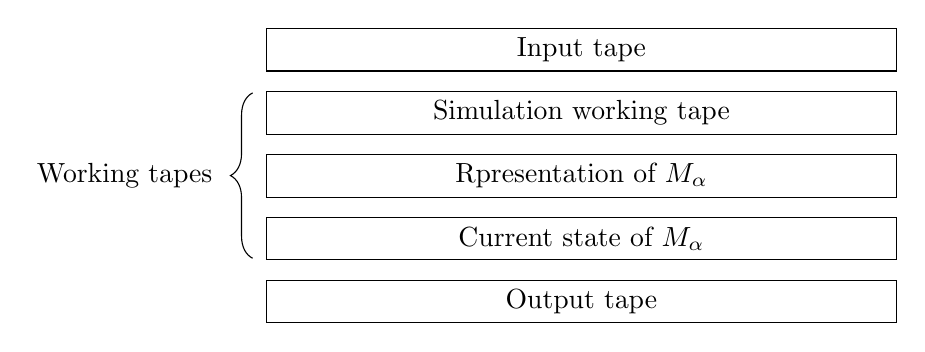
\begin{tikzpicture}
            \node[rectangle, draw, minimum width=8cm, minimum height=0.5 cm] (t1) at (0, 3.2) {Input tape};
            \node[rectangle, draw, minimum width=8cm, minimum height=0.5 cm] (t2) at (0, 2.4) {Simulation working tape};
            \node[rectangle, draw, minimum width=8cm, minimum height=0.5 cm] (t3) at (0, 1.6) {Rpresentation of $M_{\alpha}$};
            \node[rectangle, draw, minimum width=8cm, minimum height=0.5 cm] (t4) at (0, 0.8) {Current state of $M_{\alpha}$};
            \node[rectangle, draw, minimum width=8cm, minimum height=0.5 cm] (t5) at (0, 0.0) {Output tape};

            \draw[decorate, decoration={brace, raise=5pt, amplitude=8pt}] (-4, 0.55) -- (-4, 2.65) node[pos=0.5, left=16pt] {Working tapes};
        \end{tikzpicture}
        \caption{Universal Turing Machine}
        \label{fig:universal-turing-machine}
    \end{figure}
\end{proof}

\begin{rmk}
    In fact, the time bound can be improved using a more complicated encoding $\alpha$, such that if $M_{\alpha}$ halts on input $x$ within $T$ steps, then $U(x, \alpha)$ halts within $C_{\alpha}T\ln(T)$ steps for some $C_{\alpha} \in \N$.
\end{rmk}

\begin{thm}
    There exists a language that is not Turing recognizable.
\end{thm}

\begin{proof}
    Let $A$ be the set of all Turing machines, and let $L$ be the set of all languages. Since we can encode any Turing machine as a finite binary string, we can construct a bijection between the countably infinite set of finite binary strings, and $A$. Therefore $A$ is countable.

    Now, we prove that $L$ is uncountable. Consider the set $F$ of all functions from $\{0, 1\}^{*} \to \{0, 1\}$. We know that there is a bijection between $F$ and $L$, since any language can be uniquely represented as $f \in F$ such that for any finite binary string $w$, $f(w) = 1$ if and only if $w \in L$. Additionally, there is a bijection between $F$ and $[0, 1] \subset \R$. This is given by $f \in F \mapsto 0.f(w_0)f(w_1)\cdots f(w_n)\cdots \in [0, 1]$, where $w_0 = \emptystring$, $w_1 = 0$, $w_2 = 1$, $w_3 = 00$, etcetera. If $f_1 \mapsto r$ and $f_2 \mapsto r$, then $f_1(w) = f_2(w)$ for all finite binary strings $w$, and so $f_1 = f_2$. Furthermore, for any number $r \in [0, 1]$ we can explicitly construct $f$ from $r$. The necessary bijection between $[0, 1]$ and the set $T$ of all infinite binary strings, as well as the uncountability of $[0, 1]$ follows from Cantor's Diagonal Argument \ref{reals-uncountable}. We can then compose the bijections between $L$ and $F$, $F$ and $T$, and $T$ and $[0, 1]$ to obtain a bijection between $L$ and $[0, 1]$. Since $[0, 1]$ is uncountable, it follows that $L$ is as well.

    For any Turing machine $M \in A$, consider the language of all strings it recognizes. Since $A$ is countable but $L$ is not, this mapping cannot be surjective and so there exists a language that is not recognized by any Turing machine.
\end{proof}

\begin{defn}
    Consider languages $A$ and $B$. A \emph{mapping reduction} from $A$ to $B$ is a computable function $f: \Sigma^{*} \to \Sigma^{*}$ such that for any $w \in \Sigma^{*}$, $w \in A \iff f(w) \in B$. If a mapping reduction exists, we write $A \leq_{m} B$ and say that $A$ is \emph{reducible} to $B$.
\end{defn}

\begin{thm}
    Consider languages $A$ and $B$ such that $A \leq_m B$.
    \begin{itemize}
        \item If $A$ is undecidable, then $B$ is undecidable.
        \item $A$ is decidable if and only if $A$ and $\overline{A}$ are both Turing-recognizable.
    \end{itemize}
\end{thm}

\begin{exmp}
    Consider
    \begin{align*}
        A_{\textrm{TM}} &= \left\{\langle M, \alpha \rangle : \alpha \in L(M)\right\}, \\
        E_{\textrm{TM}} &= \left\{\langle M \rangle : M \textrm{ is a Turing machine, and } L(M) = \emptyset\right\}.
    \end{align*}
\end{exmp}
